\documentclass[a4paper,hidelinks,14pt]{extarticle}

\usepackage[utf8]{inputenc}
\usepackage[T2A]{fontenc}
\usepackage[english, russian]{babel}
\usepackage{amsmath}
\usepackage{amsfonts}
\usepackage{mathtools}
\usepackage{datetime}
\usepackage[pdftex]{graphicx}
\usepackage{indentfirst}
\usepackage{asymptote}
\usepackage{systeme}
\usepackage{listings}
\usepackage[usenames,dvipsnames]{color}	
\usepackage[font={small,it}]{caption}
\usepackage{gensymb}
\usepackage{hyperref}
\usepackage[framed,autolinebreaks,numbered,useliterate]{mcode}
\newcommand{\Span}{\text{Span}}
\newcommand{\Img}{\text{Im}}
\newcommand{\Ker}{\text{Ker}}
\hypersetup{
	colorlinks=true,
	linkcolor=blue,
	filecolor=magenta,      
	urlcolor=cyan,
}

\begin{document}
	\begin{titlepage}
		
		\setlength{\parindent}{0ex} % set paragraph indenting to zero
		
		\begin{center}
			\textsc{
				\vspace{1ex}
				Научно исследовательский университет ИТМО \\
				\vspace{0.5ex}
				Факультет систем управления и робототехники \\
				\vspace{0.5ex}
			}
		\end{center}
		
		\vspace{50mm}
		
		\begin{center}
			Отчет по лабораторной работе №3 \\
			Матрицы в 3D-графике
		\end{center}
		
		\vspace{50mm}
		
		\begin{minipage}{.55\linewidth}
			Выполнил студент группы R3280
			
			\smallskip
			
			Преподаватель
		\end{minipage}
		\hfill
		\begin{minipage}{.4\linewidth}
			\begin{flushright}
				Мовчан И. Е.
				\\
				Перегудин А. А.
			\end{flushright}
		\end{minipage}
		
		\vfill
		\begin{center}
			Санкт-Петербург
			\\
			2024
		\end{center}
		
	\end{titlepage}
	
	\section{Создание куба}
	С помощью кода из задания опишем куб в пространстве:
	\begin{lstlisting}
verticesCube = [
	-1,  1,  1, -1, -1,  1, 1, -1;
	-1, -1,  1,  1, -1, -1, 1,  1;
	-1, -1, -1, -1,  1,  1, 1,  1;
	1,  1,  1,  1,  1,  1, 1,  1
	];

facesCube = [
	1, 2, 6, 5;
	2, 3, 7, 6;
	3, 4, 8, 7;
	4, 1, 5, 8;
	1, 2, 3, 4;
	5, 6, 7, 8
];

DrawShape(verticesCube, facesCube, 'blue');
axis equal;
view(3);

function DrawShape(vertices, faces, color)
	patch('Vertices', (vertices(1:3,:)./vertices(4,:))', 'Faces',
   faces, 'FaceColor', color);
end
	\end{lstlisting}
	
	Использование четырехкомпонентного (четвертая координата говорит о <<весе>>) вектора мотивируется удобностью реализации смещения 3D объекта в 4D пространстве. Другие фигуры задаются через определение точек вершин (в кубическом случае за это отвечает переменная verticesCube, в которой мы задаём вершины единичного куба) и их соединение с последующим достраиванием грани через определение точек, находящихся на ней (у нас за это отвечает переменная facesCube).
	
	Функция DrawShape, на вход которой передаются массив вершин, грани и цвет, используется как обёртка для другой функции - path,  отрисовывающей трёхмерные фигуры через всё те же параметры.
	
	Строчки axis equal и view(3) указывают на то, что у нас будет выделено равно количество пространства для каждый из осей, а также на то, что мы работаем в 3D и хотим, соответственно в нём и увидеть наш результат.
	
	Запустив код, получим следующее:
	\begin{figure}[h]
		\centering
		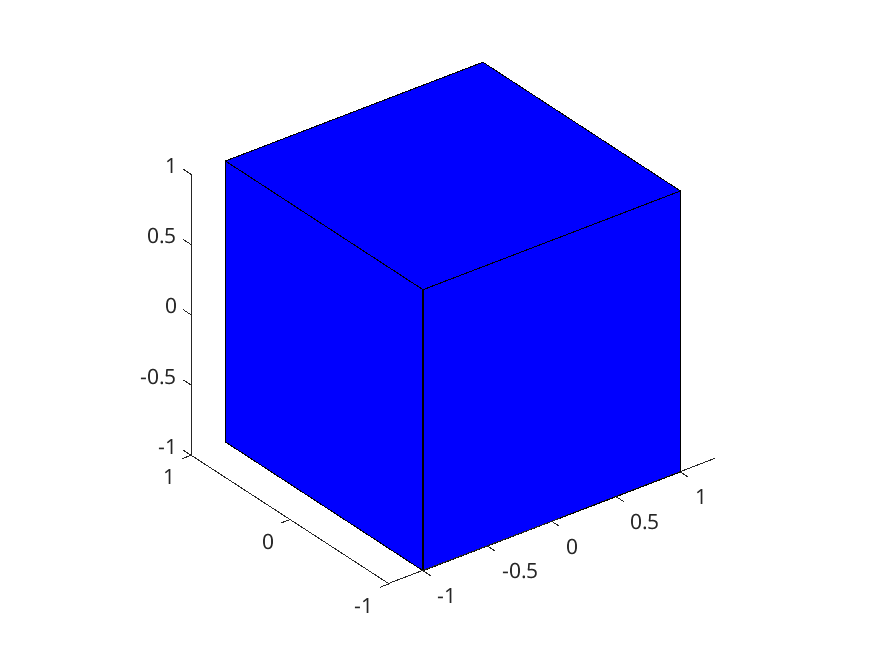
\includegraphics[scale=0.75]{./images/1.png}
		\caption{Результат работы исходного кода}
	\end{figure}
	
	Попробуем теперь немного поэксперементировать с данными. Допустим, мы захотели изменить исходные вершины единичного куба на что-то следующее:
	
	\begin{lstlisting}
verticesCube = [
	-1,  2,  1, -1, -1,  1, 1, -1;
	-1, -1,  2,  1, -1, -1, 1,  1;
	-1, -1, -1, -2,  1,  1, 1,  1;
	1,  1,  1,  1,  1,  1, 1,  1
	];
DrawShape(verticesCube, facesCube, 'blue');
	\end{lstlisting}
	
	На выходе должны будем получить что-то невнятное (так как вершины изменялись произвольным образом и не изменялись). Результат работы представлен на \ref{uncub} рисунке.
	
	\begin{figure}
		\centering
		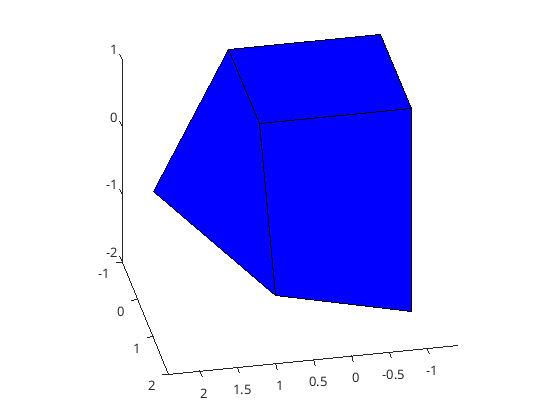
\includegraphics[scale=0.75]{./images/2.png}
		\caption{Не куб}
		\label{uncub}
	\end{figure}
	
	Таким образом, мы научились строить различные фигуры.
	
	\section{Изменение масштабов}
	Попробуем теперь немного изменить масштабы нашего куба. Матрица данного преобразования имеет следующий вид:
	\begin{lstlisting}
	Scale = [Sx,  0,  0, 0;
		      0, Sy,  0, 0;
		      0,  0, Sz, 0;
		      0,  0,  0, 1];
	\end{lstlisting}
	
	Здесь переменные Sx, Sy и Sz отвечают за растяжения/сужения по соответствующим осям. В случае простого растяжения по всем осям они будут равны. Последняя переменная не трогается, она сейчас нам не нужна.
	
	Итак, с помощью изменим код и выведем расширенный в 2 раза куб:
	\begin{lstlisting}
A1 = [2, 0, 0, 0;
	  0, 2, 0, 0;
	  0, 0, 2, 0;
	  0, 0, 0, 1];
verticesCube = A1*verticesCube;
	\end{lstlisting}
	
	Результат работы будет следующим:
	\begin{figure}[h]
		\centering
		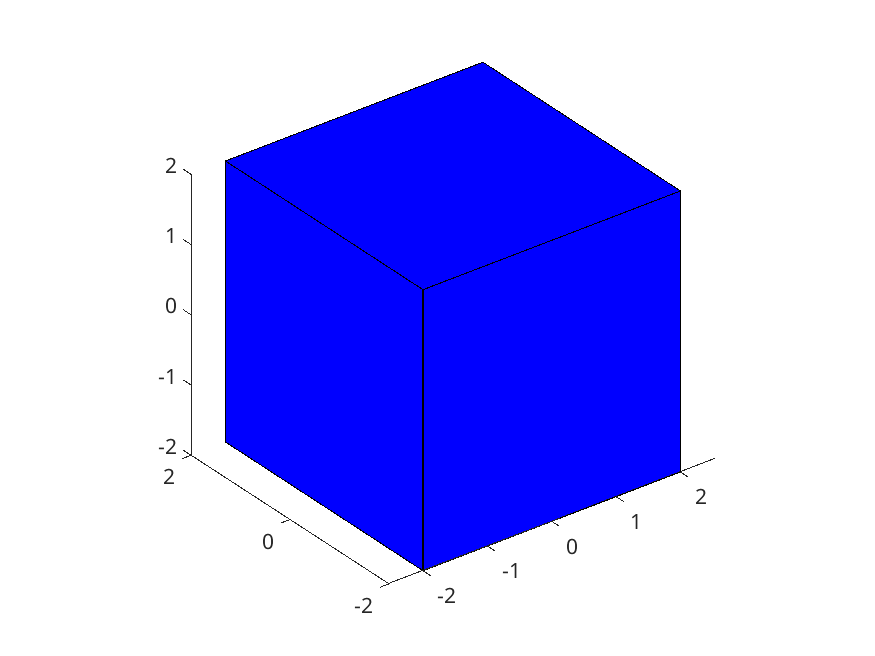
\includegraphics[scale=0.75]{./images/3.png}
		\caption{Масштабированный куб}
	\end{figure}
	
	Получили то, что и хотели! Изменим теперь масштабы только по оси Ox:
	\begin{lstlisting}
A1 = [2, 0, 0, 0;
	  0, 1, 0, 0;
	  0, 0, 1, 0;
	  0, 0, 0, 1];
verticesCube = A1*verticesCube;
	\end{lstlisting}
	
	На рисунке \ref{4} приведен результат работы. Всё получилось!
	\begin{figure}[h]
		\centering
		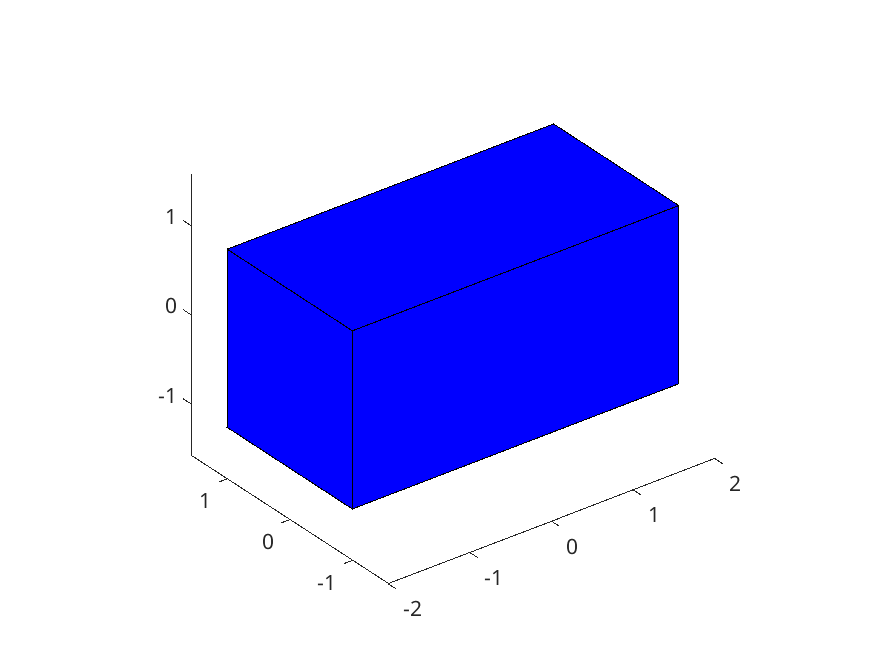
\includegraphics[scale=0.75]{./images/4.png}
		\caption{Масштабированный по Ox куб}
		\label{4}
	\end{figure}
	
	\section{Перемещение}
	Следующая матрица совершает преобразование перемещения:
	\begin{lstlisting}
A2 = [1, 0, 0, Tx;
	  0, 1, 0, Ty;
	  0, 0, 1, Tz;
	  0, 0, 0,  1];
verticesCube = A2*verticesCube;	
	\end{lstlisting}
	
	Переменные Tx, Ty и Tz отвечают за сдвиг по Ox, Oy и Oz соответственно. Здесь нам как раз требуется четвертая компонента вектора, ведь при умножении вектора на матрицу мы получаем прибавку по соответствующей оси.
	
	Посмотрим на неё в действии:
	\begin{lstlisting}
A2 = [1, 0, 0, 1;
	  0, 1, 0, 1;
	  0, 0, 1, 0;
	  0, 0, 0, 1];
verticesCube2 = A2*verticesCube;
DrawShape(verticesCube, facesCube, 'blue');
DrawShape(verticesCube2, facesCube, 'green');
	\end{lstlisting}
	
	Результат представлен на рисунке \ref{5}. Получили сдвиг, который и задавали!
	\begin{figure}[h]
		\centering
		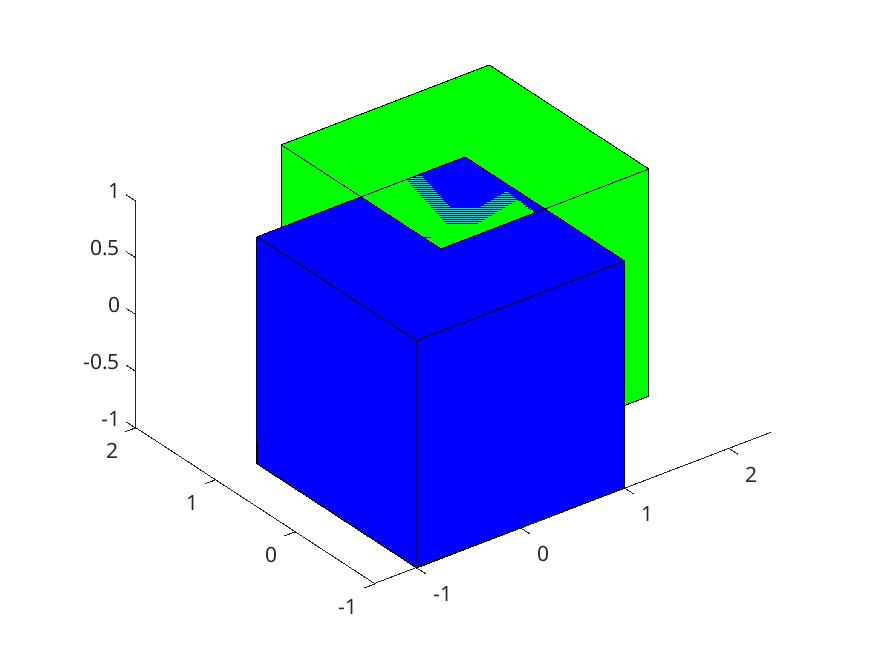
\includegraphics[scale=0.75]{./images/5.png}
		\caption{Сдвиг куба}
		\label{5}
	\end{figure}
	
	Посмотрим теперь на комбинацию преобразований перемещения и масштабирования. Зададим матрицу $A1$, растягивающую наш куб по оси Ox и Oz в 2 раза, и матрицу $A2$, делающей сдвиг центра в $(1, 1, 1)$. Композиция перемещений есть умножение матриц, а поэтому:
	\begin{lstlisting}
A1 = [2, 0, 0, 0;
	  0, 1, 0, 0;
	  0, 0, 2, 0;
	  0, 0, 0, 1];
A2 = [1, 0, 0, 1;
	  0, 1, 0, 1;
	  0, 0, 1, 1;
	  0, 0, 0, 1];
verticesCube2 = A1*A2*verticesCube;
DrawShape(verticesCube, facesCube, 'blue');
DrawShape(verticesCube2, facesCube, 'green');
	\end{lstlisting}
	
	Выполнение можем видеть на рисунке \ref{6}:
	\begin{figure}[h]
		\centering
		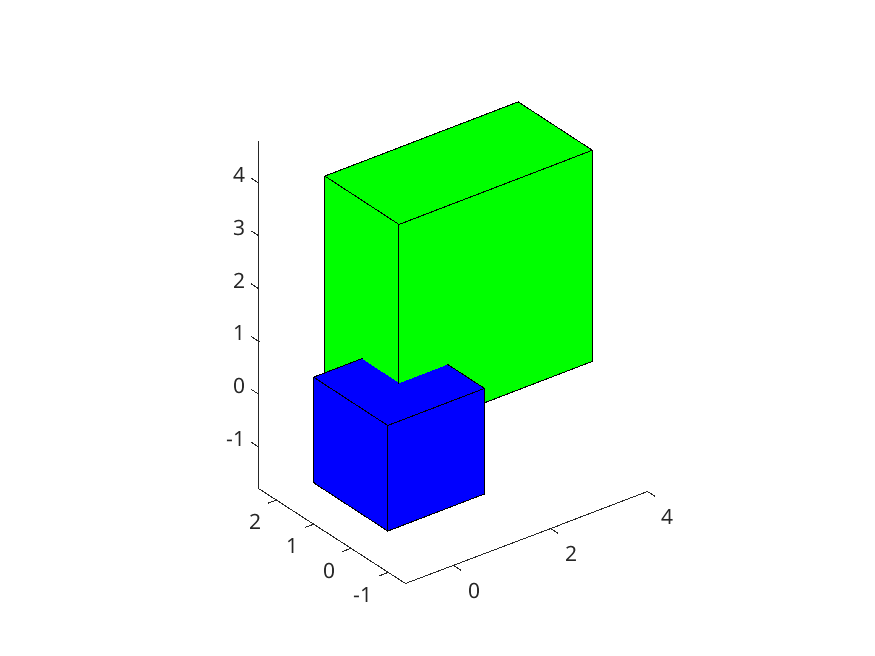
\includegraphics[scale=0.75]{./images/6.png}
		\caption{Сдвиг и масштабирование куба}
		\label{6}
	\end{figure}
	
	\section{Вращение}
	А что если мы хотим повернуть наш куб вокруг какой-то из осей? Из курса линейной алгебры мы уже знаем, как задать соответствующую матрицу, осталось лишь подействовать ею на матрицу вершин нашего куба. Хорошо, а что если мы хотим задать повернуть наш куб сначала относительно Ox, а потом относительно Oy? Всегда ли эти композиция этих преобразований оказывается равна. В 2D случае это верно в силу того, что у нас существует только одно вращение, а углы складываются (это некий вырожденный случай в мире вращений). Однако в 3D это не так:
	\begin{lstlisting}
angleOx = pi/3;
rotOx = [1,            0,             0, 0;
         0, cos(angleOx), -sin(angleOx), 0;
         0, sin(angleOx),  cos(angleOx), 0;
         0,            0,             0, 1];
angleOy = pi/6;
rotOy = [cos(angleOy), 0, sin(angleOy), 0;
		            0, 1,            0, 0;
        -sin(angleOy), 0, cos(angleOy), 0;
                    0, 0,            0, 1];
angleOz = 0;
rotOz = [cos(angleOz), -sin(angleOz), 0, 0;
		 sin(angleOz),  cos(angleOz), 0, 0;
		            0,             0, 1, 0;
		            0,             0, 0, 1];
verticesCube = rotOz*rotOx*rotOy*verticesCube;
verticesCube2 = rotOz*rotOy*rotOx*verticesCube;
	\end{lstlisting}
	
	Проверим, будут ли наши кубы совмещены:
	\begin{figure}[h]
		\centering
		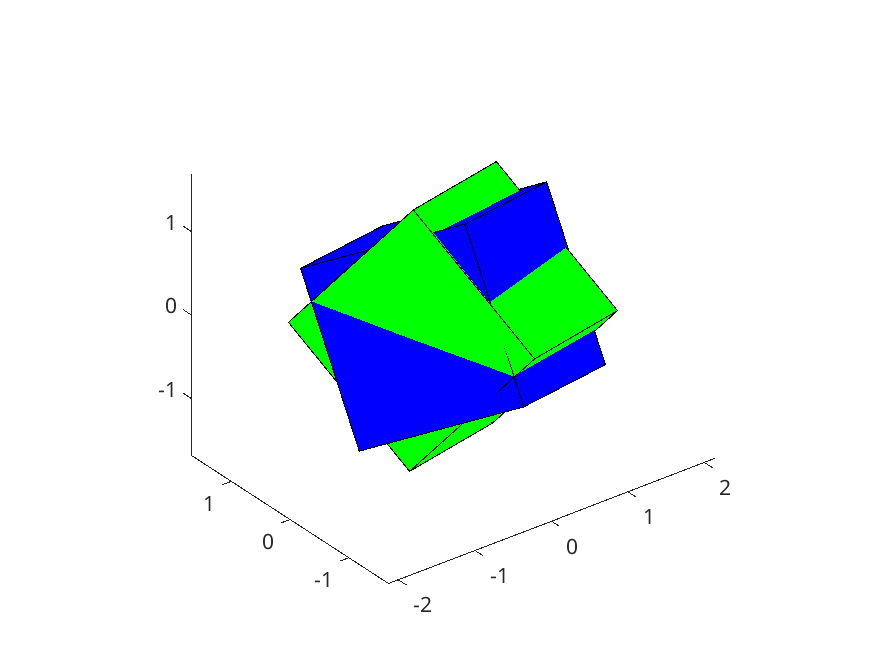
\includegraphics[scale=0.75]{./images/7.png}
		\caption{Некоммутативные вращения}
	\end{figure}
	
	То есть вращения в 3D не коммутативны. Всего же независимых вращений существует, как несложно догадаться, 3, так как независимых осей в 3D всего 3 (на то оно и 3D).
	
	\section{Вращение около одной вершины}
	Задача сводится к последовательному применению следующих преобразований: смещения вершины в центр, соответствующего поворота, а после обратного смещения в исходное положение. Приступим к реализации (будем вращать куб относительно вершины $(1, 1, 1)$):
	
	\begin{lstlisting}
A = [1, 0, 0, -1;
	 0, 1, 0, -1;
	 0, 0, 1, -1;
	 0, 0, 0, 1];
angleOx = pi/3;
rotOx = [1,            0,             0, 0;
		 0, cos(angleOx), -sin(angleOx), 0;
		 0, sin(angleOx),  cos(angleOx), 0;
		 0,            0,             0, 1];
angleOy = pi/3;
rotOy = [ cos(angleOy), 0, sin(angleOy), 0;
					 0, 1,            0, 0;
		 -sin(angleOy), 0, cos(angleOy), 0;
					 0, 0,            0, 1];
angleOz = pi/3;
rotOz = [cos(angleOz), -sin(angleOz), 0, 0;
		 sin(angleOz),  cos(angleOz), 0, 0;
					0,             0, 1, 0;
					0,             0, 0, 1];
verticesCube2 = A^(-1)*rotOz*rotOx*A*verticesCube;

DrawShape(verticesCube, facesCube, 'blue');
DrawShape(verticesCube2, facesCube, 'green');
	\end{lstlisting}
	
	Результат следующий:
	\begin{figure}[h]
		\centering
		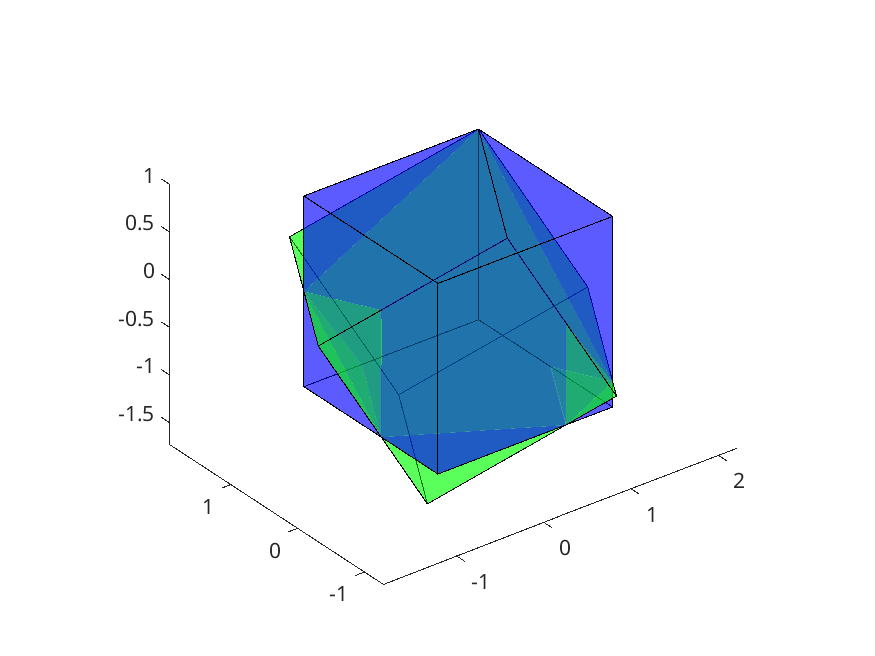
\includegraphics[scale=0.75]{./images/8.png}
		\caption{Некоммутативные вращения}
	\end{figure}
	
	Получили именно то, что мы и хотели! Заметим также, что исходная функция была немного изменена, была добавлена прозрачность $0.4$ на отрисовку с помощью добавления дополнительного аргумента FaceAlpha у функции patch.
	
	\section{Камера}
	Вооружившись всеми полученными знаниями, можем приступить к реализации камеры (точнее её симуляции, так как у нас нет неподсредственного метода её реализации). Начнём с добавления на сцену нескольких кубиков:
	\begin{lstlisting}
verticesCube = [
	-1,  1,  1, -1, -1,  1, 1, -1;
	-1, -1,  1,  1, -1, -1, 1,  1;
	-1, -1, -1, -1,  1,  1, 1,  1;
	1,  1,  1,  1,  1,  1, 1,  1
	];
		
facesCube = [
	1, 2, 6, 5;
	2, 3, 7, 6;
	3, 4, 8, 7;
	4, 1, 5, 8;
	1, 2, 3, 4;
	5, 6, 7, 8];
		
	cube1mat = [1, 0, 0, -5;
	0, 1, 0,  0;
	0, 0, 1,  0;
	0, 0, 0,  1];
		
	cube2mat = [1, 0, 0, 5;
	0, 1, 0,  1;
	0, 0, 1,  0;
	0, 0, 0,  1];
		
	cube3mat = [1, 0, 0, 0;
	0, 1, 0,  4;
	0, 0, 1,  5;
	0, 0, 0,  1];
		
	cube4mat = [1, 0, 0, 0;
	0, 1, 0,  0;
	0, 0, 1,  0;
	0, 0, 0,  1];
		
	cube1 = cube1mat*verticesCube;
	cube2 = cube2mat*verticesCube;
	cube3 = cube3mat*verticesCube;
	cube4 = cube4mat*verticesCube;
	DrawShape(cube1, facesCube, 'blue');
	DrawShape(cube2, facesCube, 'yellow');
	DrawShape(cube3, facesCube, 'green');
	DrawShape(cube4, facesCube, 'k');
		
	axis equal;
	view([0, 90]);
	function DrawShape(vertices, faces, color)
		patch('Vertices', (vertices(1:3,:)./vertices(4,:))', 'Faces', faces, 'FaceColor', color, 'FaceAlpha', 0.4);
	end
	\end{lstlisting}
	
	\begin{figure}[h]
		\centering
		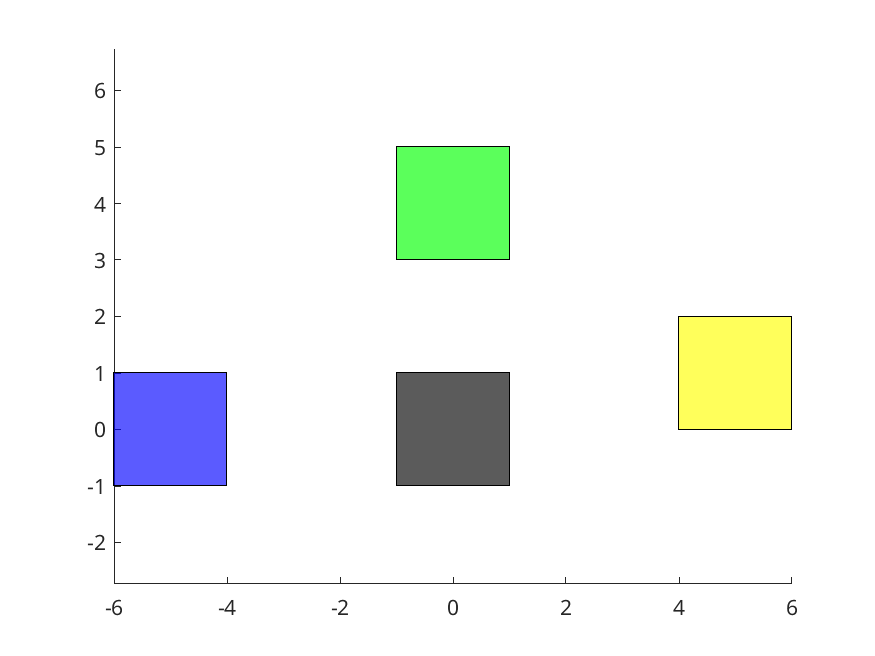
\includegraphics[scale=0.75]{./images/9.png}
		\caption{Размещение кубиков}
	\end{figure}
	
	Уже упоминалось, что у нас будет происходить не непосредственно движение камеры, а лишь её имитация, то есть если мы двигаем камеру в положительном направлении Oy на 5, то нам необходимо сместить все объекты на те же 5 пунктов в противоположном направлении, то есть взять обратную матрицу от движения камеры и применить её к объектам! Именно поэтому мы лишь моделируем движение камеры, тогда как по сути двигается не она, а сами объекты.
	
	Итак, реализуем вышеописанное движение камеры:
	\pagebreak
	\begin{lstlisting}
camera_move = [1, 0, 0, 5;
			   0, 1, 0, 0;
			   0, 0, 1, 0;
			   0, 0, 0, 1];
obj_move = camera_move^(-1);
		
cube1 = obj_move*cube1mat*verticesCube;
cube2 = obj_move*cube2mat*verticesCube;
cube3 = obj_move*cube3mat*verticesCube;
cube4 = obj_move*cube4mat*verticesCube;
DrawShape(cube1, facesCube, 'blue');
DrawShape(cube2, facesCube, 'yellow');
DrawShape(cube3, facesCube, 'green');
DrawShape(cube4, facesCube, 'k');
	\end{lstlisting}
	
	\begin{figure}[h]
		\centering
		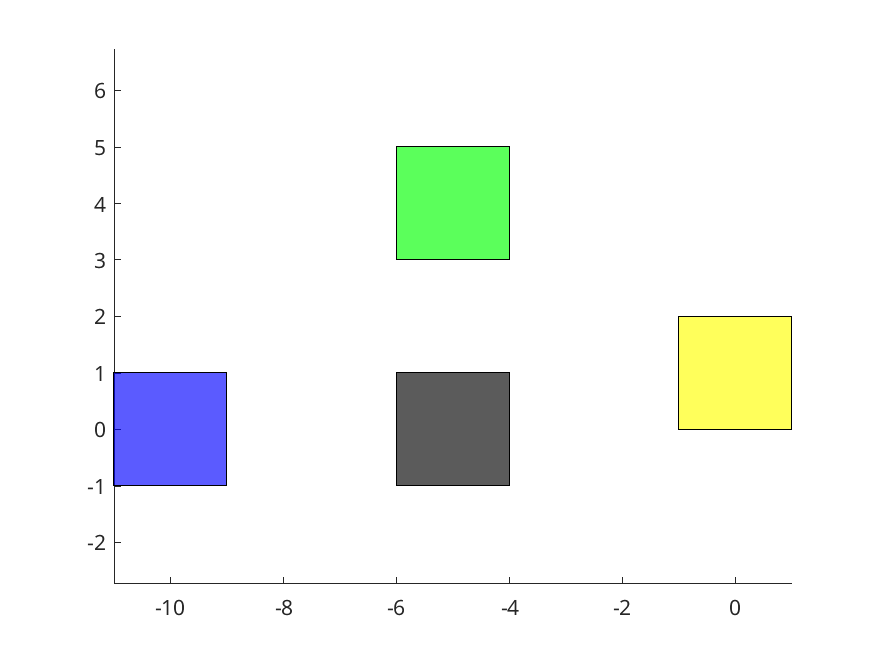
\includegraphics[scale=0.75]{./images/10.png}
		\caption{Движение камеры по Oy}
	\end{figure}
	
	Теперь повернём камеру относительно всё той же Oy, а также добавим сетку (так, мне кажется, лучше видны вращения):
	\begin{lstlisting}
camera_move = [1, 0, 0, 5;
			   0, 1, 0, 0;
			   0, 0, 1, 0;
			   0, 0, 0, 1];
angle = pi/8;
camera_rotate = [cos(angle), 0, sin(angle), 0;
						  0, 1,          0, 0;
				-sin(angle), 0, cos(angle), 0;
						  0, 0,          0, 1];
obj_move = camera_move^(-1);
obj_rotate = camera_rotate^(-1);

cube1 = obj_move*obj_rotate*cube1mat*verticesCube;
cube2 = obj_move*obj_rotate*cube2mat*verticesCube;
cube3 = obj_move*obj_rotate*cube3mat*verticesCube;
cube4 = obj_move*obj_rotate*cube4mat*verticesCube;
DrawShape(cube1, facesCube, 'blue');
DrawShape(cube2, facesCube, 'yellow');
DrawShape(cube3, facesCube, 'green');
DrawShape(cube4, facesCube, 'k');
	\end{lstlisting}
	
	\begin{figure}[h]
		\centering
		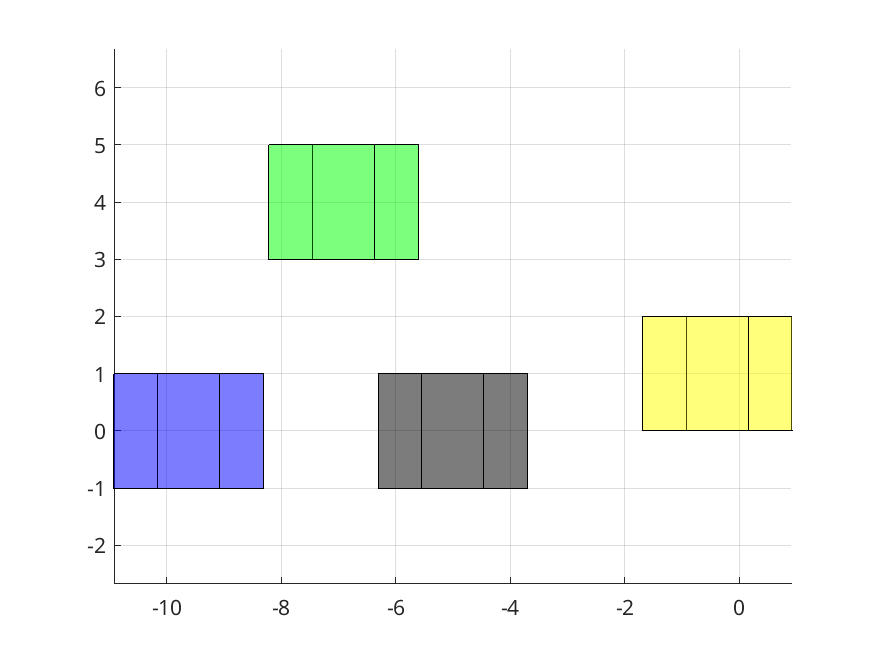
\includegraphics[scale=0.75]{./images/11.png}
		\caption{Движение и вращение камеры относительно Oy}
	\end{figure}
	
	Видим, что движения и вращения происходят успешно, всё работает!
	
	Однако не возникает такого ощущения, что наша камера выглядит как-то топорно и неестественно? С этим нам поможет справиться перспектива. 
	
	\section{Перспектива}
	Зададим следующую матрицу:
	\begin{lstlisting}
perspective = [1, 0,    0, 0;
			   0, 1,    0, 0;
		       0, 0,    1, 0;
		       0, 0, 0.04, 1];
	\end{lstlisting}
	 
	 Число в последней строке задаёт перспективное искажение при проецировании на Oxy (отрицательно число в столбце Oz дало бы искажение для поворота камеры по Ox, мы же вращаем Oy, а значит, ставим +). Чем больше это число - тем более искаженной получается картинка. Выбираем, куда ставить число, методом исключения осей, участвующих в проекции (то есть если будем проекцировать на Oxz, то число поставится в стобце Oy).
	 
	 Наши же кубы под действием этой матрицы в трёхмерном пространстве больше не будут являться таковыми. Казалось бы, одни минусы, но полученная матрица позволяет сделать нашу картинку более естественной, исказив пространство. Посмотрим на результат:
	
	\begin{figure}[h]
		\centering
		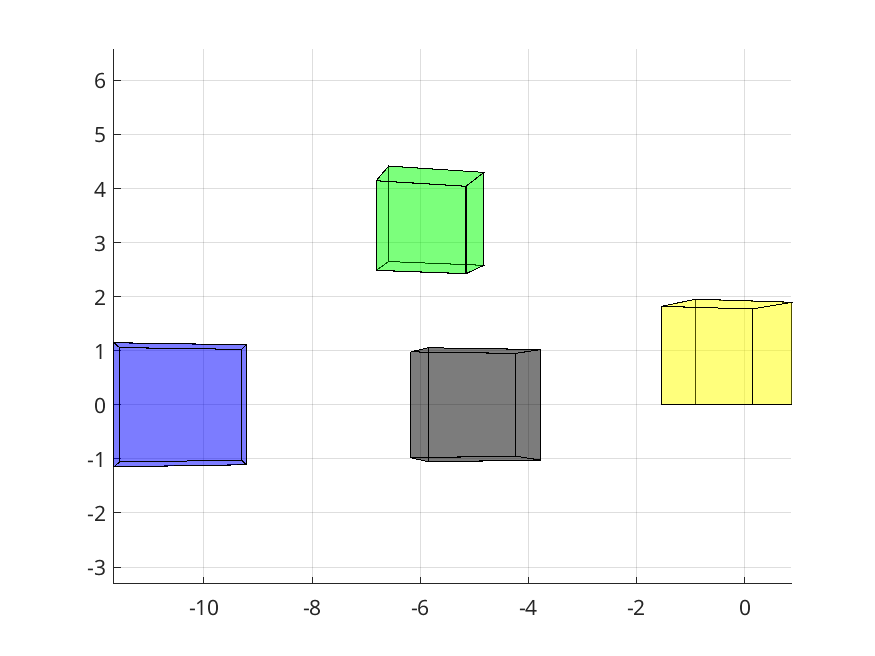
\includegraphics[scale=0.75]{./images/12.png}
		\caption{Естественное движение и вращение камеры относительно Oy}
	\end{figure}
	
	 Мы исправили проблему с неестественностью движения камеры! Теперь можем смело вращать и двигать нашу камеру, не боясь показать результаты нашей работы.
	 
	 Посмотрим теперь, что случилось с нашими кубами в пространстве:
	 \begin{figure}[h]
	 	\centering
	 	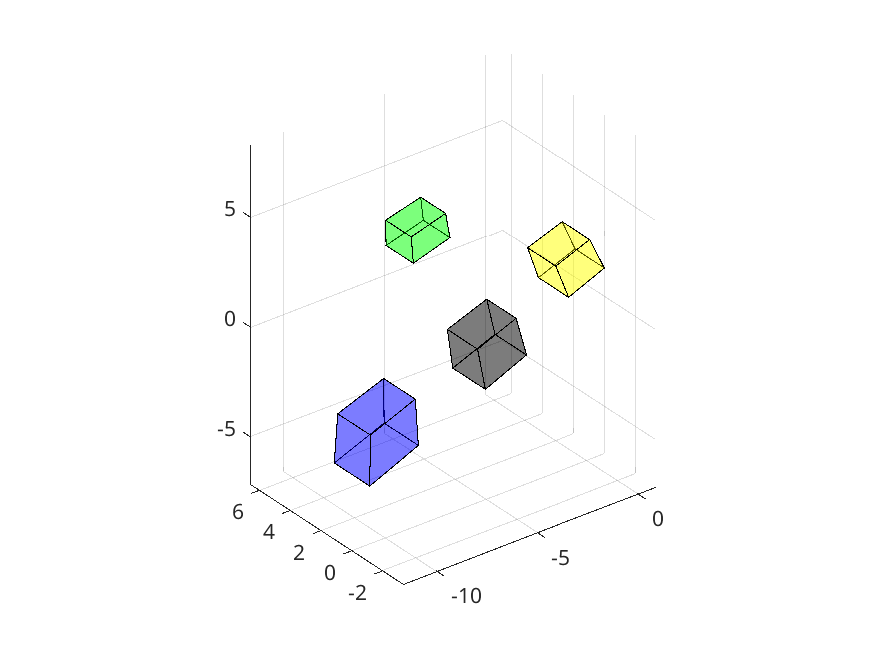
\includegraphics[scale=0.75]{./images/13.png}
	 	\caption{Искажение кубов в пространстве}
	 \end{figure}
	 
	 Как и говорилось выше, фигуры исказились, но при этом мы выиграли при проецировании в естественности движения камеры.
	 
	 \textbf{На этом всё. Спасибо!}
	
\end{document} 
